\chapter{Adaptive Step-size Selection}

So far in the course we have primarily considered algorithms with 
fixed step sizes, i.e., we assumed $t_{n} - t_{n-1} = \Delta t$ 
which is fixed. In practice, such a fixed choice is often sub-optimal 
since varying the step-size can allow us to obtain more 
efficient algorithms. 

As an example, consider the stiff ODE \eqref{eq:stiff-ODE-example}
and suppose we want to solve it using forward Euler. Since the problem 
is stiff we need to choose a very small $\Delta t$ at the beginning 
but later the solution is nice and smooth and we can choose a much 
larger value of $\Delta t$; see \Cref{fig:adaptive-forward-Euler}.
The trick to making such a method work is to allow for 
the update rules to use different step sizes, i.e., we use 
\begin{equation*}
    u_{n+1} = u_n + \Delta t_n f_n,
\end{equation*}
which is simple enough. However, the important question is 
how should we choose $\Delta t_n$? A simple approach for 
this is to try to estimate the truncation error of the 
method. In particular, for forward Euler, we recall that 
\begin{equation*}
    u(t_{n+1}) - u(t_n) + \Delta t_n f(t_n, u(t_n)) 
    = \frac{ \Delta t_n^2}{2} u''(\xi),
\end{equation*}
where $\xi \in [t_n, t_{n+1}]$.
On the other hand 
\begin{equation*}
    u''(\xi) \approx \frac{1}{\Delta t} 
    \Big( u'(t_{n+1}) - u'(t_n) \Big)
    = \frac{1}{\Delta t} \Big(
    f(t_{n+1}, u(t_{n+1})) - f(t_{n}, u(t_{n})) \Big). 
\end{equation*}
Thus, for the numerical solution, we can simply choose $\Delta t_n$ 
such that 
\begin{equation}\label{eq:l13-disp2}
    \frac{ \Delta t_n }{2} | f_{n+1} - f_n| \le \text{TOL}.
\end{equation}
This is efficient because if our proposed $\Delta t_n$ is accepted 
then we can directly use $f_{n+1}$ to compute our forward Euler step 
at no cost. 


Various strategies exist for adaptation of the 
$\Delta t_n$ that are beyond the scope of the course. A simple 
approach is to start with the error estimate 
\begin{equation*}
    \text{ERROR} =  
    \frac{ [\Delta t_n]_{\text{old}} }{2} | f_{n+1} - f_n| 
    \approx C [\Delta t_n]_{\text{old}}^2,
\end{equation*}
where we wrote $[\Delta t_n]_{\text{old}}$ to denote the step-size 
that needs to be updated.
Then we can estimate $C = \frac{\text{ERROR}}{[\Delta t_n]_{\text{old}}^2}$. 
At the same time, we want $C [\Delta t_n]_{\text{new}}^2 = \text{TOL}$, 
where we now write $[\Delta t_n]_{\text{new}}$ to denote the 
updated step-size to be chosen. 
Thus, using the estimate for $C$ we obtain a recursive formula 
to update $\Delta t_n$ at each step 
\begin{equation*}
    [\Delta t_n]_{\text{new}} \leftarrow \left( \frac{TOL}{C} \right)^{1/2}
    = [\Delta t_n]_{\text{old}} \left( \frac{TOL}{ERROR} \right)^{1/2}. 
\end{equation*}
We iterate this formula until our $\Delta t_n$ choice 
passes \eqref{eq:l13-disp2}. Note that the above 
formula has the benefit that it allows $\Delta t_n$ to 
naturally decrease but also increase should our error be 
much smaller than the tolerance.  In practice we often supplement 
this update with an extra safety parameter 
\begin{equation*}
    [\Delta t_n]_{\text{new}} \leftarrow  s \cdot [\Delta t_n]_{\text{old}} \left( \frac{TOL}{ERROR} \right)^{1/2}. 
\end{equation*}
where $s \in (0, 1]$ is a tuning parameter. 


\begin{figure}
    \centering
    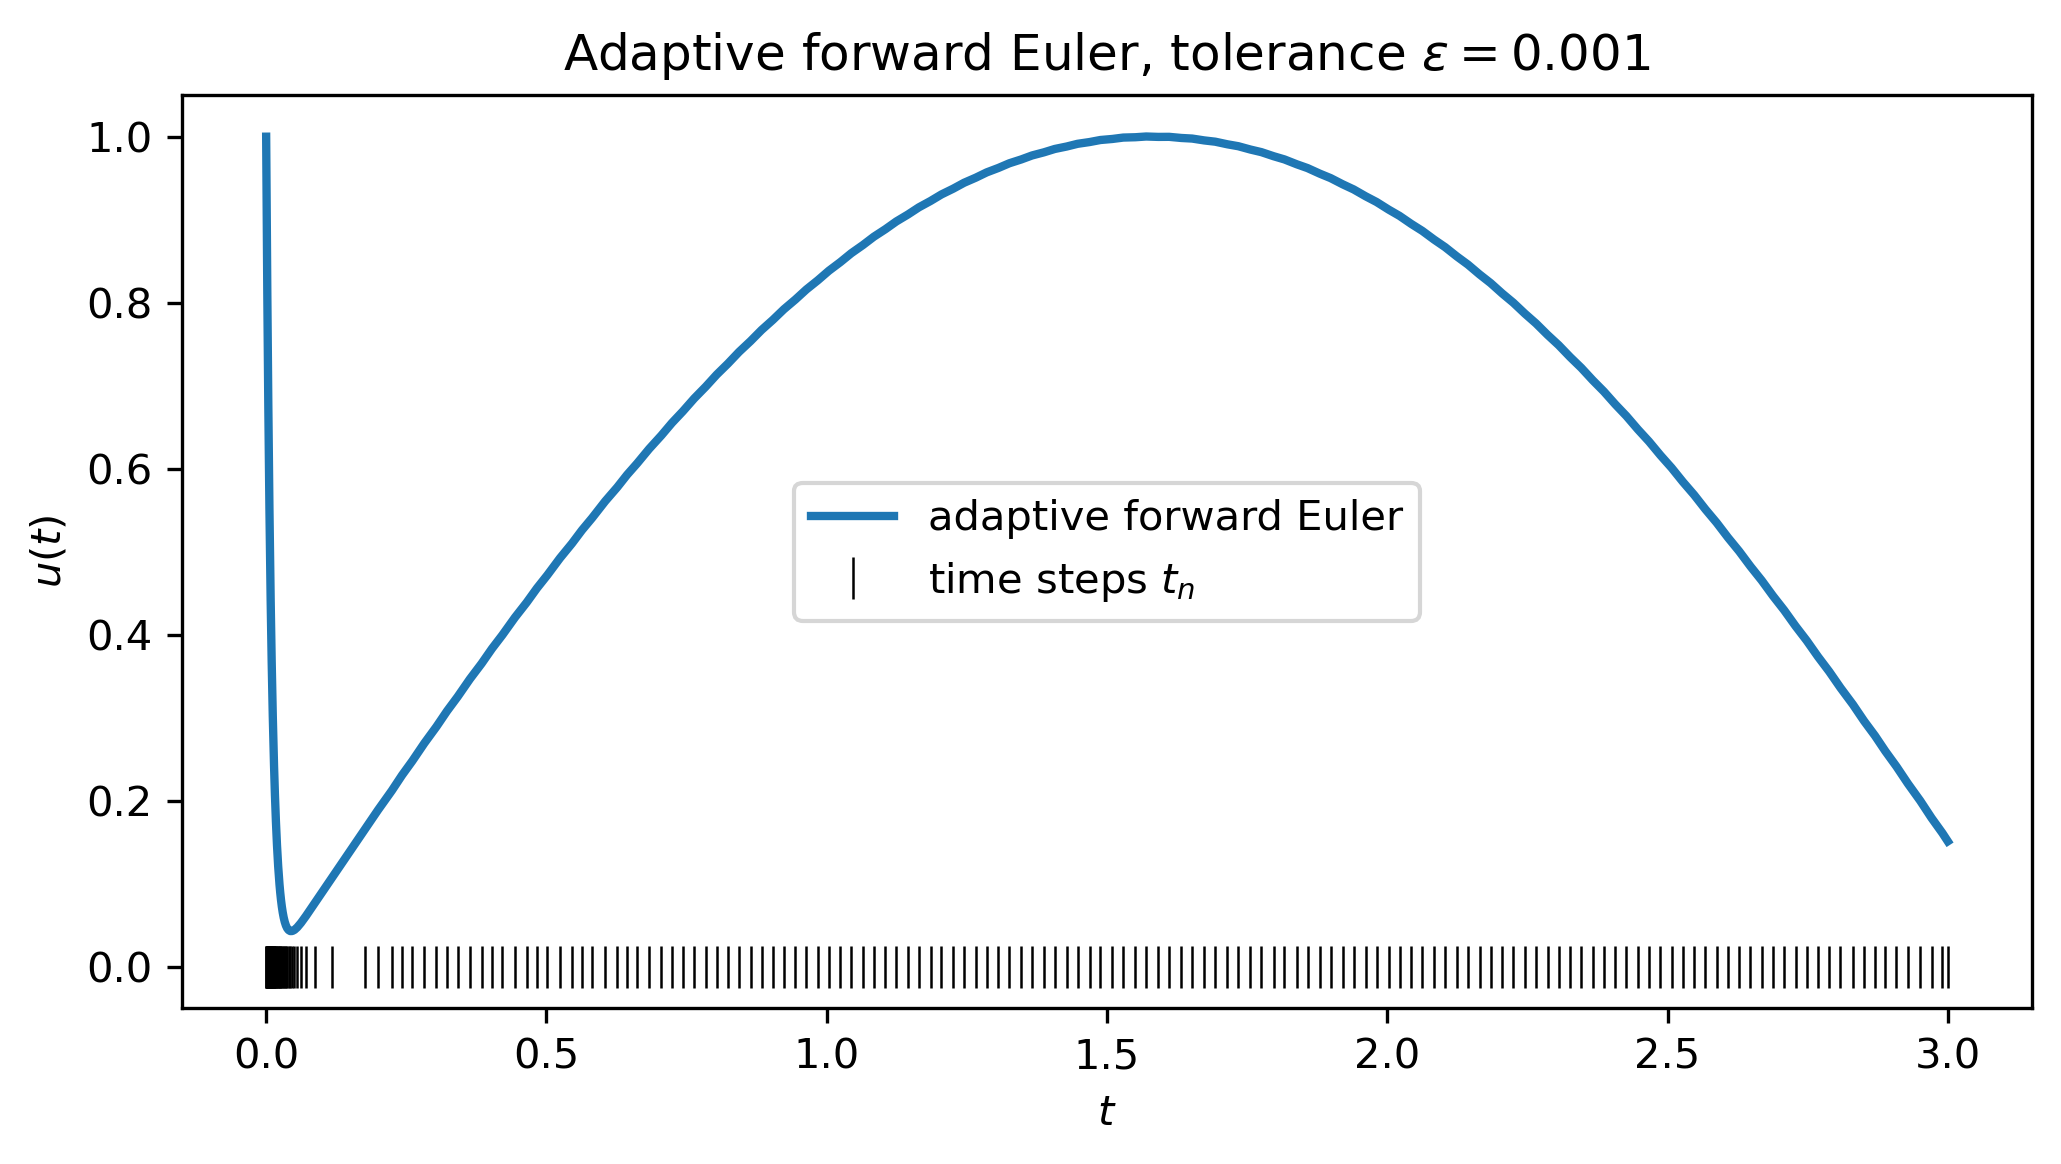
\includegraphics[width=0.6 \textwidth]{./Lectures/Lec13/adaptive_forward_euler.png}
    \caption{An instance of forward Euler with adaptive step sizes 
    chosen to control the local truncation errors below tolerance 
    $10^{-3}$.}
    \label{fig:adaptive-forward-Euler}
\end{figure}





% \bibliographystyle{plainnat}
% \bibliography{references}